% !TEX TS-program = pdflatex
\documentclass[11pt]{article}

% -------------------- Packages --------------------
\usepackage[a4paper,margin=1in]{geometry}
\usepackage{amsmath,amssymb}
\usepackage[T1]{fontenc}
\usepackage{lmodern}
\usepackage{xcolor}
\usepackage{tcolorbox}
\tcbuselibrary{skins,breakable}
\usepackage{enumitem}
\usepackage{hyperref}
\usepackage{tikz}
\usetikzlibrary{calc}

\pagestyle{empty}

% -------------------- Dark Theme Colors --------------------
\definecolor{bg}{HTML}{000000}
\definecolor{pairbg}{HTML}{121212}
\definecolor{solbg}{HTML}{0A0A0A}
\definecolor{border}{HTML}{2A2A2A}
\definecolor{text}{HTML}{FFFFFF}
\definecolor{muted}{HTML}{C9CDD3}
\definecolor{gold}{HTML}{FFD700}
\definecolor{green}{HTML}{4ADE80}
\definecolor{cyan}{HTML}{38BDF8}

\pagecolor{bg}
\color{text}

\hypersetup{
  colorlinks=true,
  linkcolor=cyan,
  urlcolor=cyan
}

\setlength{\parindent}{0pt}
\setlength{\parskip}{10pt}

\setlist[itemize]{left=1.4em,itemsep=6pt,topsep=6pt}
\setlist[enumerate]{left=1.6em,itemsep=4pt,topsep=4pt}

% -------------------- tcolorbox Base --------------------
\tcbset{
  enhanced,
  breakable,
  arc=12pt,
  boxrule=0.8pt,
  left=16pt,right=16pt,top=12pt,bottom=12pt
}

\newtcolorbox{QAPair}[1]{%
  colback=pairbg,
  colbacklower=solbg,
  colframe=border,
  coltext=text,
  title=\textcolor{gold}{\bfseries #1},
  fonttitle=\bfseries,
  coltitle=text,
  segmentation style={draw=border, dashed, line width=0.6pt},
}

\newtcolorbox{QuickBox}{%
  colback=pairbg,
  colframe=cyan,
  coltext=text,
  fontupper=\color{text},
  borderline north={4pt}{0pt}{cyan},
  arc=14pt,
  boxrule=0.8pt
}

\newcommand{\Step}[1]{\textcolor{muted}{\textbf{Step #1:}}}

% -------------------- TikZ helper styles --------------------
\tikzset{
  ubox/.style={draw=border, line width=0.9pt, fill=solbg},
  setcircle/.style={draw=text, line width=0.9pt},
  shadeG/.style={fill=green, fill opacity=0.20, draw=none},
  shadeC/.style={fill=cyan, fill opacity=0.18, draw=none},
  shadeY/.style={fill=gold, fill opacity=0.18, draw=none},
  lab/.style={text=text}
}

% ============================================================
\begin{document}

\begin{center}
{\LARGE\bfseries \textcolor{gold}{Exercise 3.1 --- Solutions}}\\[-2pt]
\end{center}

\begin{QuickBox}
{\color{cyan}\bfseries Quick formulas (Set Theory)}\par\medskip
\begin{itemize}
\item \textbf{Union:} $A\cup B=\{x: x\in A \text{ or } x\in B\}$.
\item \textbf{Intersection:} $A\cap B=\{x: x\in A \text{ and } x\in B\}$.
\item \textbf{Associative laws:} $(A\cup B)\cup C=A\cup(B\cup C)$,\quad $(A\cap B)\cap C=A\cap(B\cap C)$.
\item \textbf{Distributive laws:} $A\cup(B\cap C)=(A\cup B)\cap(A\cup C)$,\quad
$A\cap(B\cup C)=(A\cap B)\cup(A\cap C)$.
\item \textbf{Subset idea:} If $Y\subseteq X$ then $X\cup Y=X$ and $X\cap Y=Y$.
\end{itemize}
\end{QuickBox}

% ============================================================
% Q1
\begin{QAPair}{Question 1 (i)}
\textcolor{gold}{\bfseries Question:} Shade $A\cup(B\cap C)$ using diagram (i).\\
\tcblower
\textcolor{green}{\bfseries Venn diagram (shaded):}\par\medskip
\begin{center}
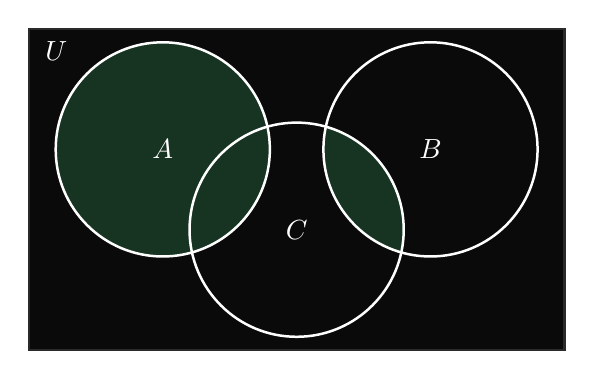
\begin{tikzpicture}[scale=0.85]
  \fill[ubox] (-4,-2.4) rectangle (4,2.4);
  \draw[ubox] (-4,-2.4) rectangle (4,2.4);
  \node[lab, anchor=north west] at (-3.9,2.35) {$U$};

  \def\r{1.6}
  \coordinate (A) at (-2,0.6);
  \coordinate (B) at ( 2,0.6);
  \coordinate (C) at ( 0,-0.6);

  % Shade: A ∪ (B ∩ C)
  \fill[shadeG] (A) circle (\r);
  \begin{scope}
    \clip (B) circle (\r);
    \fill[shadeG] (C) circle (\r);
  \end{scope}

  \draw[setcircle] (A) circle (\r);
  \draw[setcircle] (B) circle (\r);
  \draw[setcircle] (C) circle (\r);

  \node[lab] at ($(A)+(0,0)$) {$A$};
  \node[lab] at ($(B)+(0,0)$) {$B$};
  \node[lab] at ($(C)+(0,0)$) {$C$};
\end{tikzpicture}
\end{center}

\textcolor{green}{\bfseries Step-wise explanation:}
\[
\begin{aligned}
\Step{1}\;& \text{Shade }B\cap C\text{ (only the common overlap of }B\text{ and }C).\\
\Step{2}\;& \text{Shade all of }A.\\
\Step{3}\;& \text{Combine both shaded parts } \Rightarrow A\cup(B\cap C).
\end{aligned}
\]
\end{QAPair}

\begin{QAPair}{Question 1 (ii)}
\textcolor{gold}{\bfseries Question:} Shade $A\cap(B\cup C)$ using diagram (ii).\\
\tcblower
\textcolor{green}{\bfseries Venn diagram (shaded):}\par\medskip
\begin{center}
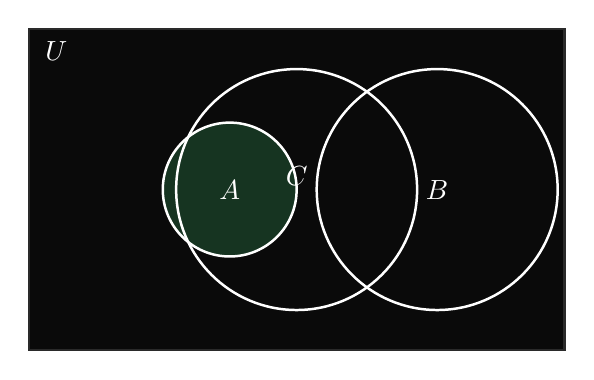
\begin{tikzpicture}[scale=0.85]
  \fill[ubox] (-4,-2.4) rectangle (4,2.4);
  \draw[ubox] (-4,-2.4) rectangle (4,2.4);
  \node[lab, anchor=north west] at (-3.9,2.35) {$U$};

  % C overlaps B; A inside C
  \def\rC{1.8}
  \def\rA{1.0}
  \def\rB{1.8}
  \coordinate (C) at (0,0);
  \coordinate (A) at (-1.0,0);
  \coordinate (B) at (2.1,0);

  % Shade: A ∩ (B ∪ C)
  \fill[shadeG] (A) circle (\rA);

  \draw[setcircle] (C) circle (\rC);
  \draw[setcircle] (A) circle (\rA);
  \draw[setcircle] (B) circle (\rB);

  \node[lab] at ($(A)+(0,0)$) {$A$};
  \node[lab] at ($(B)+(0,0)$) {$B$};
  \node[lab] at ($(C)+(0,0.2)$) {$C$};
\end{tikzpicture}
\end{center}

\textcolor{green}{\bfseries Step-wise explanation:}
\[
\begin{aligned}
\Step{1}\;& \text{First imagine shading }(B\cup C)\text{ (everything in }B\text{ or }C).\\
\Step{2}\;& \text{Now keep only the part that lies in }A \Rightarrow A\cap(B\cup C).\\
\Step{3}\;& \text{This is }(A\cap B)\cup(A\cap C)\text{ (here it becomes all of }A\text{).}
\end{aligned}
\]
\end{QAPair}

\begin{QAPair}{Question 1 (iii)}
\textcolor{gold}{\bfseries Question:} Shade $(A\cup B)\cup C$ using diagram (iii).\\
\tcblower
\textcolor{green}{\bfseries Venn diagram (shaded):}\par\medskip
\begin{center}
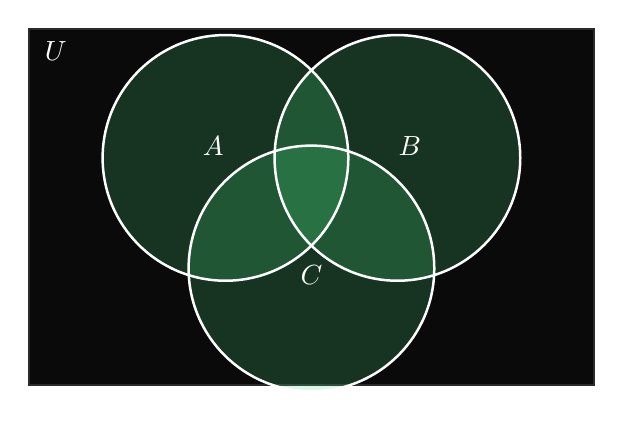
\begin{tikzpicture}[scale=0.78]
  \fill[ubox] (-4.6,-2.9) rectangle (4.6,2.9);
  \draw[ubox] (-4.6,-2.9) rectangle (4.6,2.9);
  \node[lab, anchor=north west] at (-4.5,2.85) {$U$};

  \def\r{2.0}
  \coordinate (A) at (-1.4,0.8);
  \coordinate (B) at ( 1.4,0.8);
  \coordinate (C) at ( 0,-1.0);

  \fill[shadeG] (A) circle (\r);
  \fill[shadeG] (B) circle (\r);
  \fill[shadeG] (C) circle (\r);

  \draw[setcircle] (A) circle (\r);
  \draw[setcircle] (B) circle (\r);
  \draw[setcircle] (C) circle (\r);

  \node[lab] at ($(A)+(-0.2,0.2)$) {$A$};
  \node[lab] at ($(B)+(0.2,0.2)$) {$B$};
  \node[lab] at ($(C)+(0,-0.1)$) {$C$};
\end{tikzpicture}
\end{center}

\textcolor{green}{\bfseries Step-wise explanation:}
\[
\begin{aligned}
\Step{1}\;& \text{Shade }(A\cup B)\text{ (everything in }A\text{ or }B).\\
\Step{2}\;& \text{Then union with }C:\ \text{shade all of }C\text{ as well.}\\
\Step{3}\;& \Rightarrow (A\cup B)\cup C = A\cup B\cup C.
\end{aligned}
\]
\end{QAPair}

\begin{QAPair}{Question 1 (iv)}
\textcolor{gold}{\bfseries Question:} Shade $A\cap(B\cap C)$ using diagram (iv).\\
\tcblower
\textcolor{green}{\bfseries Venn diagram (shaded):}\par\medskip
\begin{center}
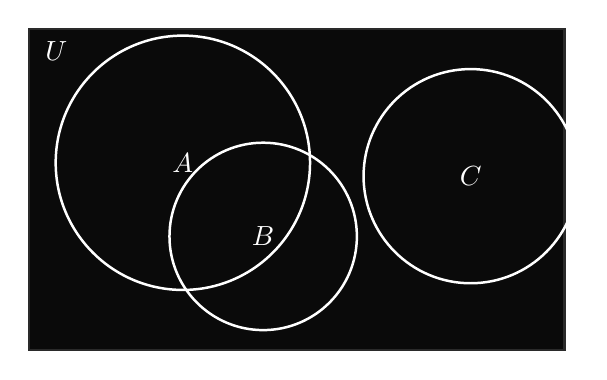
\begin{tikzpicture}[scale=0.85]
  \fill[ubox] (-4,-2.4) rectangle (4,2.4);
  \draw[ubox] (-4,-2.4) rectangle (4,2.4);
  \node[lab, anchor=north west] at (-3.9,2.35) {$U$};

  \def\rA{1.9}
  \def\rB{1.4}
  \def\rC{1.6}
  \coordinate (A) at (-1.7,0.4);
  \coordinate (B) at (-0.5,-0.7);
  \coordinate (C) at ( 2.6,0.2);

  % A∩B∩C is empty here => no shading
  \draw[setcircle] (A) circle (\rA);
  \draw[setcircle] (B) circle (\rB);
  \draw[setcircle] (C) circle (\rC);

  \node[lab] at ($(A)+(0,0)$) {$A$};
  \node[lab] at ($(B)+(0,0)$) {$B$};
  \node[lab] at ($(C)+(0,0)$) {$C$};
\end{tikzpicture}
\end{center}

\textcolor{green}{\bfseries Step-wise explanation:}
\[
\begin{aligned}
\Step{1}\;& B\cap C\ \text{means ``common part of }B\text{ and }C\text{''.}\\
\Step{2}\;& A\cap(B\cap C)=A\cap B\cap C\ \text{(triple common part).}\\
\Step{3}\;& \text{Here }C\text{ does not overlap }A\text{ or }B \Rightarrow A\cap B\cap C=\varnothing.\\
\Step{4}\;& \text{So nothing is shaded.}
\end{aligned}
\]
\end{QAPair}

% ============================================================
% Q2
\begin{QAPair}{Question 2}
\textcolor{gold}{\bfseries Question:}
If $X=\{a,b,c,d,e\}$, $Y=\{a,c,e\}$, $Z=\{g,h,i,j\}$, find the following using Venn diagram:
(i) $(X\cup Y)\cup Z$ \;
(ii) $X\cup (Y\cup Z)$ \;
(iii) $(X\cap Y)\cap Z$ \;
(iv) $X\cap(Y\cap Z)$ \;
(v) $(X\cup Y)\cap Z$ \;
(vi) $(X\cap Y)\cup Z$.\\
\tcblower

\textcolor{green}{\bfseries Venn diagram (elements placed):}\par\medskip
\begin{center}
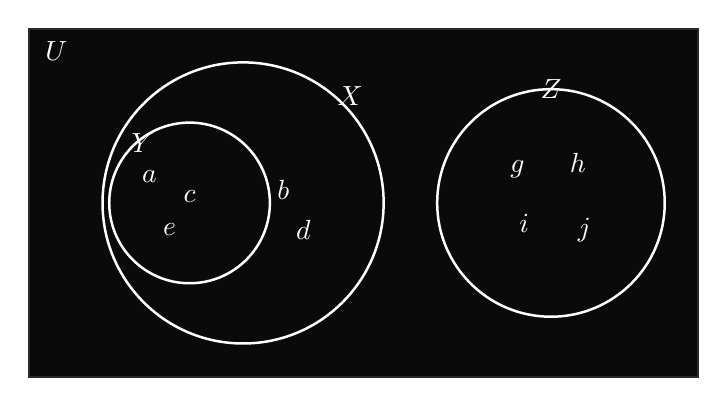
\begin{tikzpicture}[scale=0.85]
  \fill[ubox] (-5,-2.6) rectangle (5,2.6);
  \draw[ubox] (-5,-2.6) rectangle (5,2.6);
  \node[lab, anchor=north west] at (-4.9,2.55) {$U$};

  \coordinate (X) at (-1.8,0.0);
  \coordinate (Y) at (-2.6,0.0);
  \coordinate (Z) at ( 2.8,0.0);
  \def\rX{2.1}
  \def\rY{1.2}
  \def\rZ{1.7}

  \draw[setcircle] (X) circle (\rX);
  \draw[setcircle] (Y) circle (\rY);
  \draw[setcircle] (Z) circle (\rZ);

  \node[lab] at ($(X)+(1.6,1.6)$) {$X$};
  \node[lab] at ($(Y)+(-0.7,0.9)$) {$Y$};
  \node[lab] at ($(Z)+(0.0,1.7)$) {$Z$};

  \node[lab] at (-3.2,0.4) {$a$};
  \node[lab] at (-2.6,0.1) {$c$};
  \node[lab] at (-2.9,-0.4) {$e$};

  \node[lab] at (-1.2,0.2) {$b$};
  \node[lab] at (-0.9,-0.4) {$d$};

  \node[lab] at (2.3,0.5) {$g$};
  \node[lab] at (3.2,0.6) {$h$};
  \node[lab] at (2.4,-0.3) {$i$};
  \node[lab] at (3.3,-0.4) {$j$};
\end{tikzpicture}
\end{center}

\textcolor{green}{\bfseries Answer:}
\[
\begin{aligned}
\Step{1}\;& Y\subseteq X \Rightarrow X\cup Y=X,\quad X\cap Y=Y.\\
\Step{2}\;& (i)\ (X\cup Y)\cup Z = X\cup Z=\{a,b,c,d,e,g,h,i,j\}.\\
\Step{3}\;& (ii)\ X\cup(Y\cup Z)=X\cup Z=\{a,b,c,d,e,g,h,i,j\}.\\
\Step{4}\;& (iii)\ (X\cap Y)\cap Z=Y\cap Z=\varnothing.\\
\Step{5}\;& (iv)\ X\cap(Y\cap Z)=X\cap\varnothing=\varnothing.\\
\Step{6}\;& (v)\ (X\cup Y)\cap Z=X\cap Z=\varnothing.\\
\Step{7}\;& (vi)\ (X\cap Y)\cup Z=Y\cup Z=\{a,c,e,g,h,i,j\}.
\end{aligned}
\]
\end{QAPair}

% ============================================================
% Q3 (UPDATED: step-wise)
\begin{QAPair}{Question 3}
\textcolor{gold}{\bfseries Question:} Verify associative law of union and intersection by using diagrams of Question 1.\\
\tcblower

\textcolor{green}{\bfseries (A) Associative law of union: $(A\cup B)\cup C=A\cup(B\cup C)$}\par
\[
\begin{aligned}
\Step{1}\;& \text{Shade }A\cup B\text{ (everything in }A\text{ or }B).\\
\Step{2}\;& \text{Union with }C:\ \text{shade all of }C\ \Rightarrow (A\cup B)\cup C.\\
\Step{3}\;& \text{Now shade }B\cup C\text{ first, then union with }A.\\
\Step{4}\;& \text{In both ways, the shaded region is }A\cup B\cup C.
\end{aligned}
\]

\textcolor{green}{\bfseries Union diagram (both sides give the same shading):}\par\medskip
\begin{center}
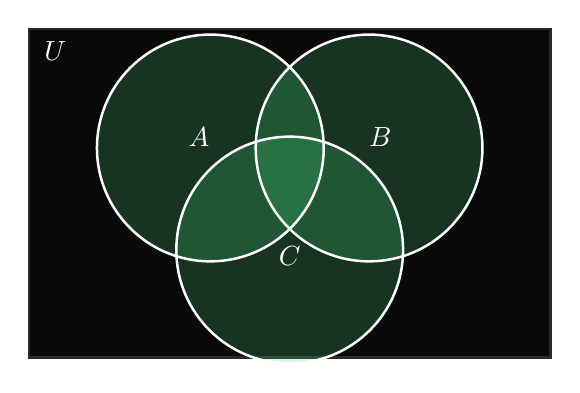
\begin{tikzpicture}[scale=0.72]
  \fill[ubox] (-4.6,-2.9) rectangle (4.6,2.9);
  \draw[ubox] (-4.6,-2.9) rectangle (4.6,2.9);
  \node[lab, anchor=north west] at (-4.5,2.85) {$U$};

  \def\r{2.0}
  \coordinate (A) at (-1.4,0.8);
  \coordinate (B) at ( 1.4,0.8);
  \coordinate (C) at ( 0,-1.0);

  \fill[shadeG] (A) circle (\r);
  \fill[shadeG] (B) circle (\r);
  \fill[shadeG] (C) circle (\r);

  \draw[setcircle] (A) circle (\r);
  \draw[setcircle] (B) circle (\r);
  \draw[setcircle] (C) circle (\r);

  \node[lab] at ($(A)+(-0.2,0.2)$) {$A$};
  \node[lab] at ($(B)+(0.2,0.2)$) {$B$};
  \node[lab] at ($(C)+(0,-0.1)$) {$C$};
\end{tikzpicture}
\end{center}

\textcolor{green}{\bfseries (B) Associative law of intersection: $(A\cap B)\cap C=A\cap(B\cap C)$}\par
\[
\begin{aligned}
\Step{1}\;& \text{Shade }A\cap B\text{ (only the overlap of }A\text{ and }B).\\
\Step{2}\;& \text{Intersect with }C:\ \text{keep only the part that is also in }C.\\
\Step{3}\;& \text{Alternatively, shade }B\cap C\text{ first, then keep only the part in }A.\\
\Step{4}\;& \text{Both give the same final region: }A\cap B\cap C.
\end{aligned}
\]

\textcolor{green}{\bfseries Intersection diagram (triple overlap):}\par\medskip
\begin{center}
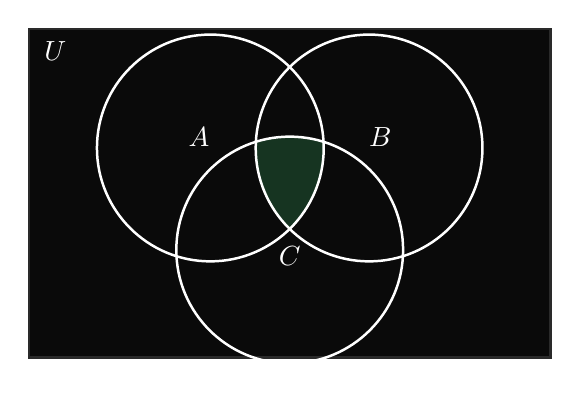
\begin{tikzpicture}[scale=0.72]
  \fill[ubox] (-4.6,-2.9) rectangle (4.6,2.9);
  \draw[ubox] (-4.6,-2.9) rectangle (4.6,2.9);
  \node[lab, anchor=north west] at (-4.5,2.85) {$U$};

  \def\r{2.0}
  \coordinate (A) at (-1.4,0.8);
  \coordinate (B) at ( 1.4,0.8);
  \coordinate (C) at ( 0,-1.0);

  \begin{scope}
    \clip (A) circle (\r);
    \clip (B) circle (\r);
    \fill[shadeG] (C) circle (\r);
  \end{scope}

  \draw[setcircle] (A) circle (\r);
  \draw[setcircle] (B) circle (\r);
  \draw[setcircle] (C) circle (\r);

  \node[lab] at ($(A)+(-0.2,0.2)$) {$A$};
  \node[lab] at ($(B)+(0.2,0.2)$) {$B$};
  \node[lab] at ($(C)+(0,-0.1)$) {$C$};
\end{tikzpicture}
\end{center}

\textcolor{green}{\bfseries Conclusion:}
\[
(A\cup B)\cup C=A\cup(B\cup C),\qquad (A\cap B)\cap C=A\cap(B\cap C).
\]
\end{QAPair}

% ============================================================
% Q4 (UPDATED: step-wise)
\begin{QAPair}{Question 4}
\textcolor{gold}{\bfseries Question:} Verify distributive laws using Venn diagrams:
(i) $A\cup(B\cap C)=(A\cup B)\cap(A\cup C)$,
(ii) $A\cap(B\cup C)=(A\cap B)\cup(A\cap C)$.\\
\tcblower

\textcolor{green}{\bfseries (i) Verify $A\cup(B\cap C)=(A\cup B)\cap(A\cup C)$}\par
\[
\begin{aligned}
\Step{1}\;& \text{LHS: shade }B\cap C,\ \text{then shade all of }A,\ \text{combine (union).}\\
\Step{2}\;& \text{RHS: shade }(A\cup B)\ \text{and shade }(A\cup C).\\
\Step{3}\;& \text{The common (overlapped) part of these two shaded regions is the RHS.}\\
\Step{4}\;& \text{Both diagrams give the same final region, so the identity is verified.}
\end{aligned}
\]

\begin{center}
\begin{minipage}{0.48\linewidth}
\centering
\textcolor{muted}{LHS: $A\cup(B\cap C)$}\par\smallskip
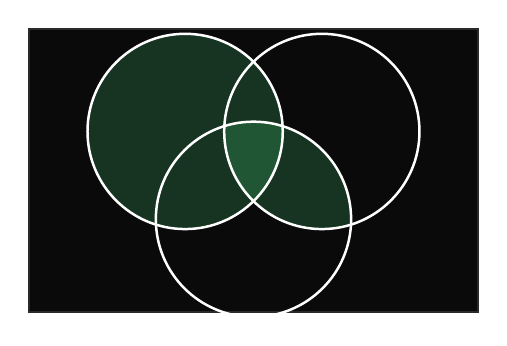
\begin{tikzpicture}[scale=0.62]
  \fill[ubox] (-4.6,-2.9) rectangle (4.6,2.9);
  \draw[ubox] (-4.6,-2.9) rectangle (4.6,2.9);

  \def\r{2.0}
  \coordinate (A) at (-1.4,0.8);
  \coordinate (B) at ( 1.4,0.8);
  \coordinate (C) at ( 0,-1.0);

  % shade A plus (B∩C)
  \fill[shadeG] (A) circle (\r);
  \begin{scope}
    \clip (B) circle (\r);
    \fill[shadeG] (C) circle (\r);
  \end{scope}

  \draw[setcircle] (A) circle (\r);
  \draw[setcircle] (B) circle (\r);
  \draw[setcircle] (C) circle (\r);
\end{tikzpicture}
\end{minipage}\hfill
\begin{minipage}{0.48\linewidth}
\centering
\textcolor{muted}{RHS: $(A\cup B)\cap(A\cup C)$}\par\smallskip
\textcolor{muted}{(overlap of two shadings)}\par\smallskip
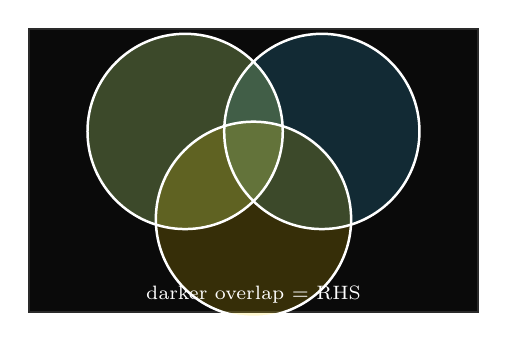
\begin{tikzpicture}[scale=0.62]
  \fill[ubox] (-4.6,-2.9) rectangle (4.6,2.9);
  \draw[ubox] (-4.6,-2.9) rectangle (4.6,2.9);

  \def\r{2.0}
  \coordinate (A) at (-1.4,0.8);
  \coordinate (B) at ( 1.4,0.8);
  \coordinate (C) at ( 0,-1.0);

  % Shade union1 = A∪B (cyan)
  \fill[shadeC] (A) circle (\r);
  \fill[shadeC] (B) circle (\r);

  % Shade union2 = A∪C (gold)
  \fill[shadeY] (A) circle (\r);
  \fill[shadeY] (C) circle (\r);

  % Outlines
  \draw[setcircle] (A) circle (\r);
  \draw[setcircle] (B) circle (\r);
  \draw[setcircle] (C) circle (\r);

  \node[lab] at (0,-2.55) {\scriptsize darker overlap = RHS};
\end{tikzpicture}
\end{minipage}
\end{center}

\textcolor{green}{\bfseries (ii) Verify $A\cap(B\cup C)=(A\cap B)\cup(A\cap C)$}\par
\[
\begin{aligned}
\Step{1}\;& \text{LHS: shade }(B\cup C),\ \text{then keep only the part inside }A.\\
\Step{2}\;& \text{That produces two pieces: }(A\cap B)\ \text{and }(A\cap C).\\
\Step{3}\;& \text{RHS: shade }(A\cap B)\ \text{and shade }(A\cap C)\ \text{and take their union.}\\
\Step{4}\;& \text{Both sides shade the same region, so the identity is verified.}
\end{aligned}
\]

\begin{center}
\begin{minipage}{0.48\linewidth}
\centering
\textcolor{muted}{LHS: $A\cap(B\cup C)$}\par\smallskip
\textcolor{muted}{(overlap of $A$ with $B\cup C$)}\par\smallskip
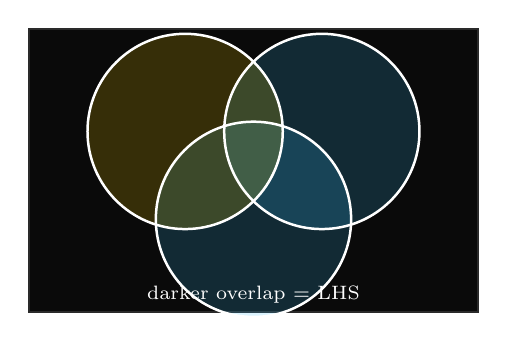
\begin{tikzpicture}[scale=0.62]
  \fill[ubox] (-4.6,-2.9) rectangle (4.6,2.9);
  \draw[ubox] (-4.6,-2.9) rectangle (4.6,2.9);

  \def\r{2.0}
  \coordinate (A) at (-1.4,0.8);
  \coordinate (B) at ( 1.4,0.8);
  \coordinate (C) at ( 0,-1.0);

  % Shade (B∪C) cyan
  \fill[shadeC] (B) circle (\r);
  \fill[shadeC] (C) circle (\r);

  % Shade A gold (the overlap is LHS)
  \fill[shadeY] (A) circle (\r);

  \draw[setcircle] (A) circle (\r);
  \draw[setcircle] (B) circle (\r);
  \draw[setcircle] (C) circle (\r);

  \node[lab] at (0,-2.55) {\scriptsize darker overlap = LHS};
\end{tikzpicture}
\end{minipage}\hfill
\begin{minipage}{0.48\linewidth}
\centering
\textcolor{muted}{RHS: $(A\cap B)\cup(A\cap C)$}\par\smallskip
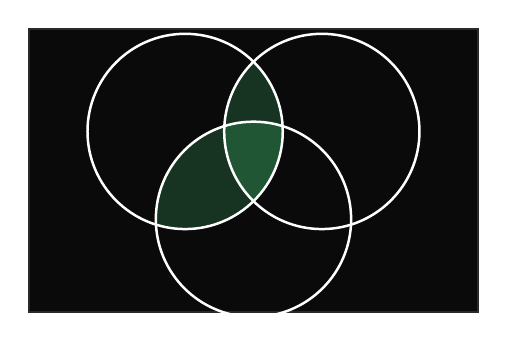
\begin{tikzpicture}[scale=0.62]
  \fill[ubox] (-4.6,-2.9) rectangle (4.6,2.9);
  \draw[ubox] (-4.6,-2.9) rectangle (4.6,2.9);

  \def\r{2.0}
  \coordinate (A) at (-1.4,0.8);
  \coordinate (B) at ( 1.4,0.8);
  \coordinate (C) at ( 0,-1.0);

  % Shade (A∩B)
  \begin{scope}
    \clip (A) circle (\r);
    \fill[shadeG] (B) circle (\r);
  \end{scope}
  % Shade (A∩C)
  \begin{scope}
    \clip (A) circle (\r);
    \fill[shadeG] (C) circle (\r);
  \end{scope}

  \draw[setcircle] (A) circle (\r);
  \draw[setcircle] (B) circle (\r);
  \draw[setcircle] (C) circle (\r);
\end{tikzpicture}
\end{minipage}
\end{center}
\end{QAPair}

% ============================================================
% Q5 (UPDATED: include Venn diagrams)
\begin{QAPair}{Question 5}
\textcolor{gold}{\bfseries Question:} Prove by using Venn diagram:
(a) $(P\cup Q)\cup R = P\cup(Q\cup R)$,\;
(b) $(P\cap Q)\cap R = P\cap(Q\cap R)$,\\
when\\
(i) $P=\{0,1,2,3\}$,\ $Q=\{2,3,4,5,6\}$,\ $R=\{5,6,7,8,9\}$\\
(ii) $P=\{m,n,o,p,q\}$,\ $Q=\{r,s,t,u\}$,\ $R=\{t,u,v,w\}$.\\
\tcblower

\textcolor{green}{\bfseries (i) Venn diagrams with elements}\par\medskip
\begin{center}
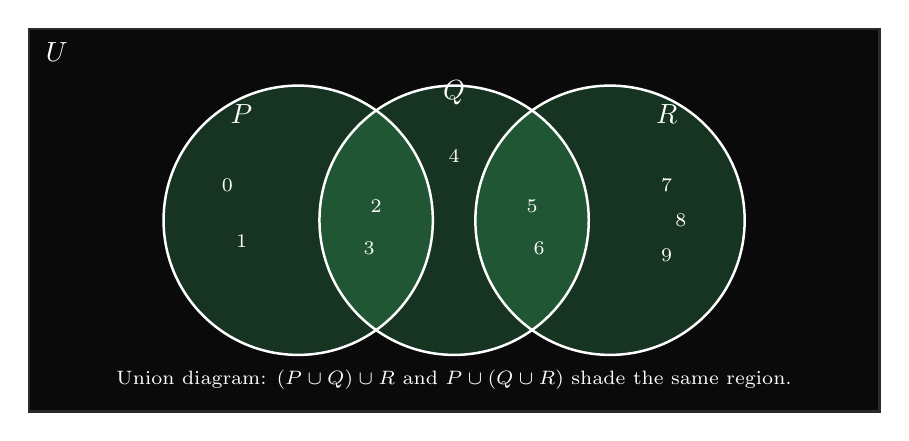
\begin{tikzpicture}[scale=0.90]
  \fill[ubox] (-6,-2.7) rectangle (6,2.7);
  \draw[ubox] (-6,-2.7) rectangle (6,2.7);
  \node[lab, anchor=north west] at (-5.9,2.65) {$U$};

  % Chain-style: P overlaps Q, Q overlaps R, P and R disjoint
  \def\r{1.9}
  \coordinate (P) at (-2.2,0);
  \coordinate (Q) at ( 0.0,0);
  \coordinate (R) at ( 2.2,0);

  % (a) Union shading: all three circles (this represents both sides)
  \fill[shadeG] (P) circle (\r);
  \fill[shadeG] (Q) circle (\r);
  \fill[shadeG] (R) circle (\r);

  \draw[setcircle] (P) circle (\r);
  \draw[setcircle] (Q) circle (\r);
  \draw[setcircle] (R) circle (\r);

  \node[lab] at ($(P)+(-0.8,1.5)$) {$P$};
  \node[lab] at ($(Q)+(0.0,1.8)$) {$Q$};
  \node[lab] at ($(R)+(0.8,1.5)$) {$R$};

  % Place elements
  \node[lab] at (-3.2,0.5) {\scriptsize $0$};
  \node[lab] at (-3.0,-0.3) {\scriptsize $1$};

  \node[lab] at (-1.1,0.2) {\scriptsize $2$};
  \node[lab] at (-1.2,-0.4) {\scriptsize $3$};

  \node[lab] at (0.0,0.9) {\scriptsize $4$};

  \node[lab] at (1.1,0.2) {\scriptsize $5$};
  \node[lab] at (1.2,-0.4) {\scriptsize $6$};

  \node[lab] at (3.0,0.5) {\scriptsize $7$};
  \node[lab] at (3.2,0.0) {\scriptsize $8$};
  \node[lab] at (3.0,-0.5) {\scriptsize $9$};

  \node[lab] at (0,-2.25) {\scriptsize Union diagram: $(P\cup Q)\cup R$ and $P\cup(Q\cup R)$ shade the same region.};
\end{tikzpicture}
\end{center}

\textcolor{green}{\bfseries Step-wise verification (i):}
\[
\begin{aligned}
\Step{1}\;& P\cup Q=\{0,1,2,3,4,5,6\}.\\
\Step{2}\;& (P\cup Q)\cup R=\{0,1,2,3,4,5,6,7,8,9\}.\\
\Step{3}\;& Q\cup R=\{2,3,4,5,6,7,8,9\}.\\
\Step{4}\;& P\cup(Q\cup R)=\{0,1,2,3,4,5,6,7,8,9\}.\\
\Step{5}\;& \Rightarrow (P\cup Q)\cup R = P\cup(Q\cup R).\\[4pt]
\Step{6}\;& P\cap Q=\{2,3\},\ Q\cap R=\{5,6\},\ P\cap R=\varnothing.\\
\Step{7}\;& (P\cap Q)\cap R=\varnothing,\quad P\cap(Q\cap R)=\varnothing.\\
\Step{8}\;& \Rightarrow (P\cap Q)\cap R = P\cap(Q\cap R).
\end{aligned}
\]

\textcolor{green}{\bfseries (ii) Venn diagram (structure + elements)}\par\medskip
\begin{center}
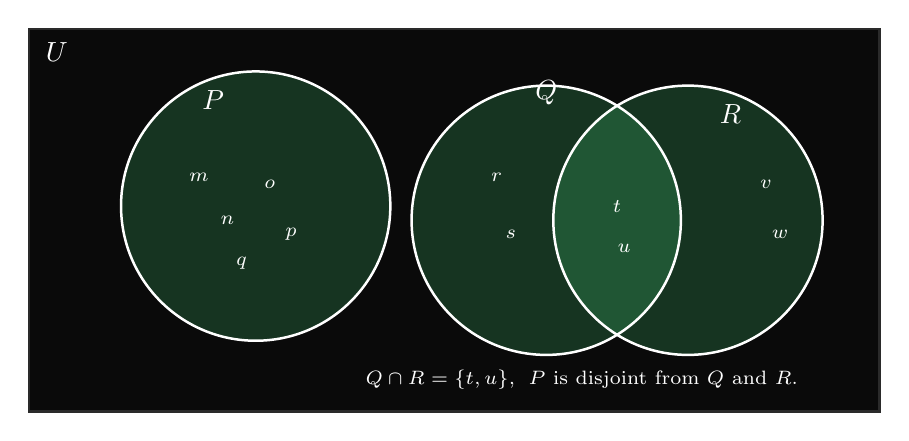
\begin{tikzpicture}[scale=0.90]
  \fill[ubox] (-6,-2.7) rectangle (6,2.7);
  \draw[ubox] (-6,-2.7) rectangle (6,2.7);
  \node[lab, anchor=north west] at (-5.9,2.65) {$U$};

  \def\r{1.9}
  \coordinate (Q) at ( 1.3,0);
  \coordinate (R) at ( 3.3,0);
  \coordinate (P) at (-2.8,0.2);

  % Union shading (same for both sides of union identity)
  \fill[shadeG] (P) circle (\r);
  \fill[shadeG] (Q) circle (\r);
  \fill[shadeG] (R) circle (\r);

  \draw[setcircle] (P) circle (\r);
  \draw[setcircle] (Q) circle (\r);
  \draw[setcircle] (R) circle (\r);

  \node[lab] at ($(P)+(-0.6,1.5)$) {$P$};
  \node[lab] at ($(Q)+(0.0,1.8)$) {$Q$};
  \node[lab] at ($(R)+(0.6,1.5)$) {$R$};

  % Place elements
  \node[lab] at (-3.6,0.6) {\scriptsize $m$};
  \node[lab] at (-3.2,0.0) {\scriptsize $n$};
  \node[lab] at (-2.6,0.5) {\scriptsize $o$};
  \node[lab] at (-2.3,-0.2) {\scriptsize $p$};
  \node[lab] at (-3.0,-0.6) {\scriptsize $q$};

  \node[lab] at (0.6,0.6) {\scriptsize $r$};
  \node[lab] at (0.8,-0.2) {\scriptsize $s$};

  \node[lab] at (2.3,0.2) {\scriptsize $t$};
  \node[lab] at (2.4,-0.4) {\scriptsize $u$};

  \node[lab] at (4.4,0.5) {\scriptsize $v$};
  \node[lab] at (4.6,-0.2) {\scriptsize $w$};

  \node[lab] at (1.8,-2.25) {\scriptsize $Q\cap R=\{t,u\}$,\; $P$ is disjoint from $Q$ and $R$.};
\end{tikzpicture}
\end{center}

\textcolor{green}{\bfseries Step-wise verification (ii):}
\[
\begin{aligned}
\Step{1}\;& (P\cup Q)\cup R=\{m,n,o,p,q,r,s,t,u,v,w\}.\\
\Step{2}\;& P\cup(Q\cup R)=\{m,n,o,p,q,r,s,t,u,v,w\}.\\
\Step{3}\;& P\cap Q=\varnothing \Rightarrow (P\cap Q)\cap R=\varnothing.\\
\Step{4}\;& Q\cap R=\{t,u\},\ \text{but }P\cap(Q\cap R)=\varnothing.\\
\Step{5}\;& \Rightarrow \text{Both associative laws hold.}
\end{aligned}
\]
\end{QAPair}

% ============================================================
% Q6 (UPDATED: include Venn diagrams)
\begin{QAPair}{Question 6}
\textcolor{gold}{\bfseries Question:} Verify $X\cup(Y\cap Z)=(X\cup Y)\cap(X\cup Z)$ for\\
$X=\{-1,-2,-3\}$,\ $Y=\{0,1,2,3\}$,\ $Z=\{0,\pm 1,\pm 2,\pm 3\}$.\\
\tcblower

\textcolor{green}{\bfseries Key observation:} $X\subseteq Z$ and $Y\subseteq Z$ (both are inside $Z$), and $X\cap Y=\varnothing$.\\

\textcolor{green}{\bfseries Step-wise verification:}
\[
\begin{aligned}
\Step{1}\;& Y\cap Z=Y \quad (\text{because }Y\subseteq Z).\\
\Step{2}\;& X\cup(Y\cap Z)=X\cup Y=\{-3,-2,-1,0,1,2,3\}.\\
\Step{3}\;& X\cup Z=Z \quad (\text{because }X\subseteq Z).\\
\Step{4}\;& (X\cup Y)\cap(X\cup Z)=(X\cup Y)\cap Z=X\cup Y.\\
\Step{5}\;& \Rightarrow\ \text{LHS}=\text{RHS. Verified.}
\end{aligned}
\]

\textcolor{green}{\bfseries Venn diagrams (both sides shade the same region):}\par\medskip
\begin{center}
\begin{minipage}{0.48\linewidth}
\centering
\textcolor{muted}{LHS: $X\cup(Y\cap Z)=X\cup Y$}\par\smallskip
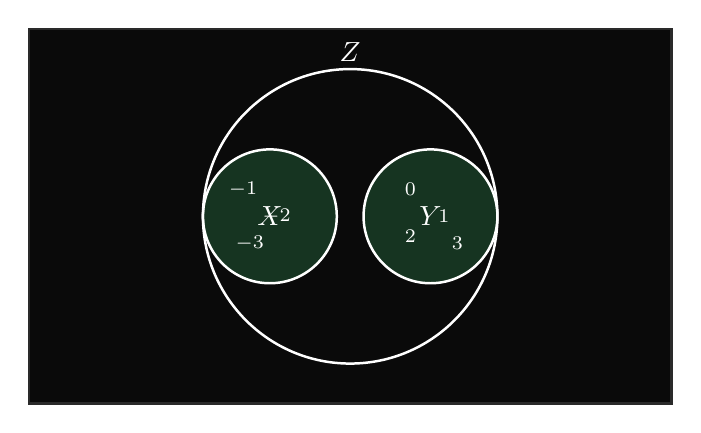
\begin{tikzpicture}[scale=0.85]
  \fill[ubox] (-4.8,-2.8) rectangle (4.8,2.8);
  \draw[ubox] (-4.8,-2.8) rectangle (4.8,2.8);

  % Z big circle, X and Y inside disjoint
  \coordinate (Z) at (0,0);
  \coordinate (X) at (-1.2,0);
  \coordinate (Y) at ( 1.2,0);
  \def\rZ{2.2}
  \def\rS{1.0}

  % Shade X and Y (i.e., X ∪ Y)
  \fill[shadeG] (X) circle (\rS);
  \fill[shadeG] (Y) circle (\rS);

  \draw[setcircle] (Z) circle (\rZ);
  \draw[setcircle] (X) circle (\rS);
  \draw[setcircle] (Y) circle (\rS);

  \node[lab] at (0,2.45) {$Z$};
  \node[lab] at (-1.2,0.0) {$X$};
  \node[lab] at ( 1.2,0.0) {$Y$};

  % Elements
  \node[lab] at (-1.6,0.4) {\scriptsize $-1$};
  \node[lab] at (-1.1,0.0) {\scriptsize $-2$};
  \node[lab] at (-1.5,-0.4) {\scriptsize $-3$};

  \node[lab] at ( 0.9,0.4) {\scriptsize $0$};
  \node[lab] at ( 1.4,0.0) {\scriptsize $1$};
  \node[lab] at ( 0.9,-0.3) {\scriptsize $2$};
  \node[lab] at ( 1.6,-0.4) {\scriptsize $3$};
\end{tikzpicture}
\end{minipage}\hfill
\begin{minipage}{0.48\linewidth}
\centering
\textcolor{muted}{RHS: $(X\cup Y)\cap(X\cup Z)$}\par\smallskip
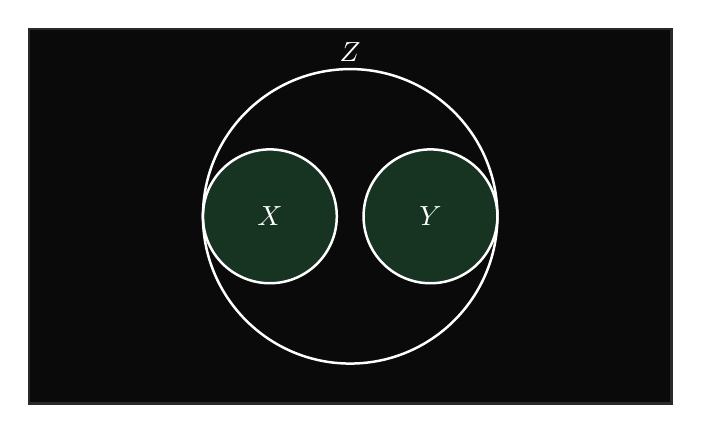
\begin{tikzpicture}[scale=0.85]
  \fill[ubox] (-4.8,-2.8) rectangle (4.8,2.8);
  \draw[ubox] (-4.8,-2.8) rectangle (4.8,2.8);

  \coordinate (Z) at (0,0);
  \coordinate (X) at (-1.2,0);
  \coordinate (Y) at ( 1.2,0);
  \def\rZ{2.2}
  \def\rS{1.0}

  % Since X∪Z = Z, intersection keeps (X∪Y) inside Z, i.e. X∪Y
  \fill[shadeG] (X) circle (\rS);
  \fill[shadeG] (Y) circle (\rS);

  \draw[setcircle] (Z) circle (\rZ);
  \draw[setcircle] (X) circle (\rS);
  \draw[setcircle] (Y) circle (\rS);

  \node[lab] at (0,2.45) {$Z$};
  \node[lab] at (-1.2,0.0) {$X$};
  \node[lab] at ( 1.2,0.0) {$Y$};
\end{tikzpicture}
\end{minipage}
\end{center}
\end{QAPair}

% ============================================================
% Q7 (UPDATED: include Venn diagrams)
\begin{QAPair}{Question 7}
\textcolor{gold}{\bfseries Question:} Verify $X\cap(Y\cup Z)=(X\cap Y)\cup(X\cap Z)$ where\\
$X=$ set of first three vowels,\ $Y=$ set of letters of ``energy'',\ $Z=$ set of letters of ``algebra''.\\
\tcblower

\textcolor{green}{\bfseries Step-wise verification:}
\[
\begin{aligned}
\Step{1}\;& X=\{a,e,i\}.\\
\Step{2}\;& Y=\{e,n,r,g,y\}.\\
\Step{3}\;& Z=\{a,l,g,e,b,r\}.\\
\Step{4}\;& Y\cup Z=\{a,b,e,g,l,n,r,y\}.\\
\Step{5}\;& X\cap(Y\cup Z)=\{a,e\}.\\
\Step{6}\;& X\cap Y=\{e\},\quad X\cap Z=\{a,e\}.\\
\Step{7}\;& (X\cap Y)\cup(X\cap Z)=\{e\}\cup\{a,e\}=\{a,e\}.\\
\Step{8}\;& \Rightarrow\ \text{LHS}=\text{RHS. Verified.}
\end{aligned}
\]

\textcolor{green}{\bfseries Venn diagrams (both sides shade the same region):}\par\medskip
\begin{center}
\begin{minipage}{0.48\linewidth}
\centering
\textcolor{muted}{LHS: $X\cap(Y\cup Z)$}\par\smallskip
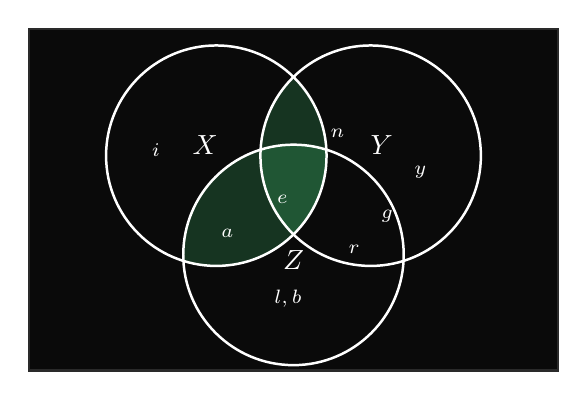
\begin{tikzpicture}[scale=0.70]
  \fill[ubox] (-4.8,-3.1) rectangle (4.8,3.1);
  \draw[ubox] (-4.8,-3.1) rectangle (4.8,3.1);

  \def\r{2.0}
  \coordinate (X) at (-1.4,0.8);
  \coordinate (Y) at ( 1.4,0.8);
  \coordinate (Z) at ( 0,-1.0);

  % Shade region = parts of X that are in (Y or Z)
  % This equals (X∩Y) ∪ (X∩Z): shade X∩Y and X∩Z
  \begin{scope}
    \clip (X) circle (\r);
    \fill[shadeG] (Y) circle (\r);
  \end{scope}
  \begin{scope}
    \clip (X) circle (\r);
    \fill[shadeG] (Z) circle (\r);
  \end{scope}

  \draw[setcircle] (X) circle (\r);
  \draw[setcircle] (Y) circle (\r);
  \draw[setcircle] (Z) circle (\r);

  \node[lab] at ($(X)+(-0.2,0.2)$) {$X$};
  \node[lab] at ($(Y)+(0.2,0.2)$) {$Y$};
  \node[lab] at ($(Z)+(0,-0.1)$) {$Z$};

  % Place letters
  \node[lab] at (-2.5,0.9) {\scriptsize $i$};        % only in X
  \node[lab] at (-0.2,0.0) {\scriptsize $e$};        % in X∩Y∩Z
  \node[lab] at (-1.2,-0.6) {\scriptsize $a$};       % in X∩Z only
  \node[lab] at (0.8,1.2) {\scriptsize $n$};         % only in Y
  \node[lab] at (2.3,0.5) {\scriptsize $y$};         % only in Y
  \node[lab] at (1.7,-0.3) {\scriptsize $g$};        % in Y∩Z
  \node[lab] at (1.1,-0.9) {\scriptsize $r$};        % in Y∩Z
  \node[lab] at (-0.1,-1.8) {\scriptsize $l,b$};     % only in Z
\end{tikzpicture}
\end{minipage}\hfill
\begin{minipage}{0.48\linewidth}
\centering
\textcolor{muted}{RHS: $(X\cap Y)\cup(X\cap Z)$}\par\smallskip
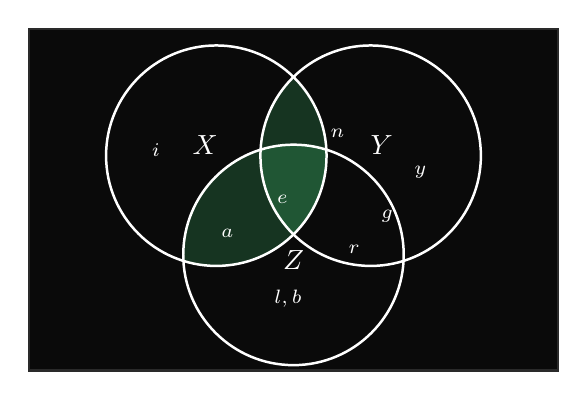
\begin{tikzpicture}[scale=0.70]
  \fill[ubox] (-4.8,-3.1) rectangle (4.8,3.1);
  \draw[ubox] (-4.8,-3.1) rectangle (4.8,3.1);

  \def\r{2.0}
  \coordinate (X) at (-1.4,0.8);
  \coordinate (Y) at ( 1.4,0.8);
  \coordinate (Z) at ( 0,-1.0);

  % Shade (X∩Y)
  \begin{scope}
    \clip (X) circle (\r);
    \fill[shadeG] (Y) circle (\r);
  \end{scope}
  % Shade (X∩Z)
  \begin{scope}
    \clip (X) circle (\r);
    \fill[shadeG] (Z) circle (\r);
  \end{scope}

  \draw[setcircle] (X) circle (\r);
  \draw[setcircle] (Y) circle (\r);
  \draw[setcircle] (Z) circle (\r);

  \node[lab] at ($(X)+(-0.2,0.2)$) {$X$};
  \node[lab] at ($(Y)+(0.2,0.2)$) {$Y$};
  \node[lab] at ($(Z)+(0,-0.1)$) {$Z$};

  \node[lab] at (-2.5,0.9) {\scriptsize $i$};
  \node[lab] at (-0.2,0.0) {\scriptsize $e$};
  \node[lab] at (-1.2,-0.6) {\scriptsize $a$};
  \node[lab] at (0.8,1.2) {\scriptsize $n$};
  \node[lab] at (2.3,0.5) {\scriptsize $y$};
  \node[lab] at (1.7,-0.3) {\scriptsize $g$};
  \node[lab] at (1.1,-0.9) {\scriptsize $r$};
  \node[lab] at (-0.1,-1.8) {\scriptsize $l,b$};
\end{tikzpicture}
\end{minipage}
\end{center}

\textcolor{green}{\bfseries Final shaded set in both diagrams:} $\{a,e\}$.
\end{QAPair}

\end{document}
